\section{Streamlining the build process}
Before this project began PIPE 4's build process had not changed since it was first developed; it was hosted on SourceForge and made use of CVS for its version control. We migrated the project to Git and transferred the project from SourceForge to GitHub because GitHub provides a richer variety of developer tools including issue tracking (\cref{fig:gh_issues}), forking, easy releases, continuous-integration (\cref{fig:travis_ci}) and the support of a project website.

\mediumlinespacing
\begin{figure}[tb]
\begin{center}
    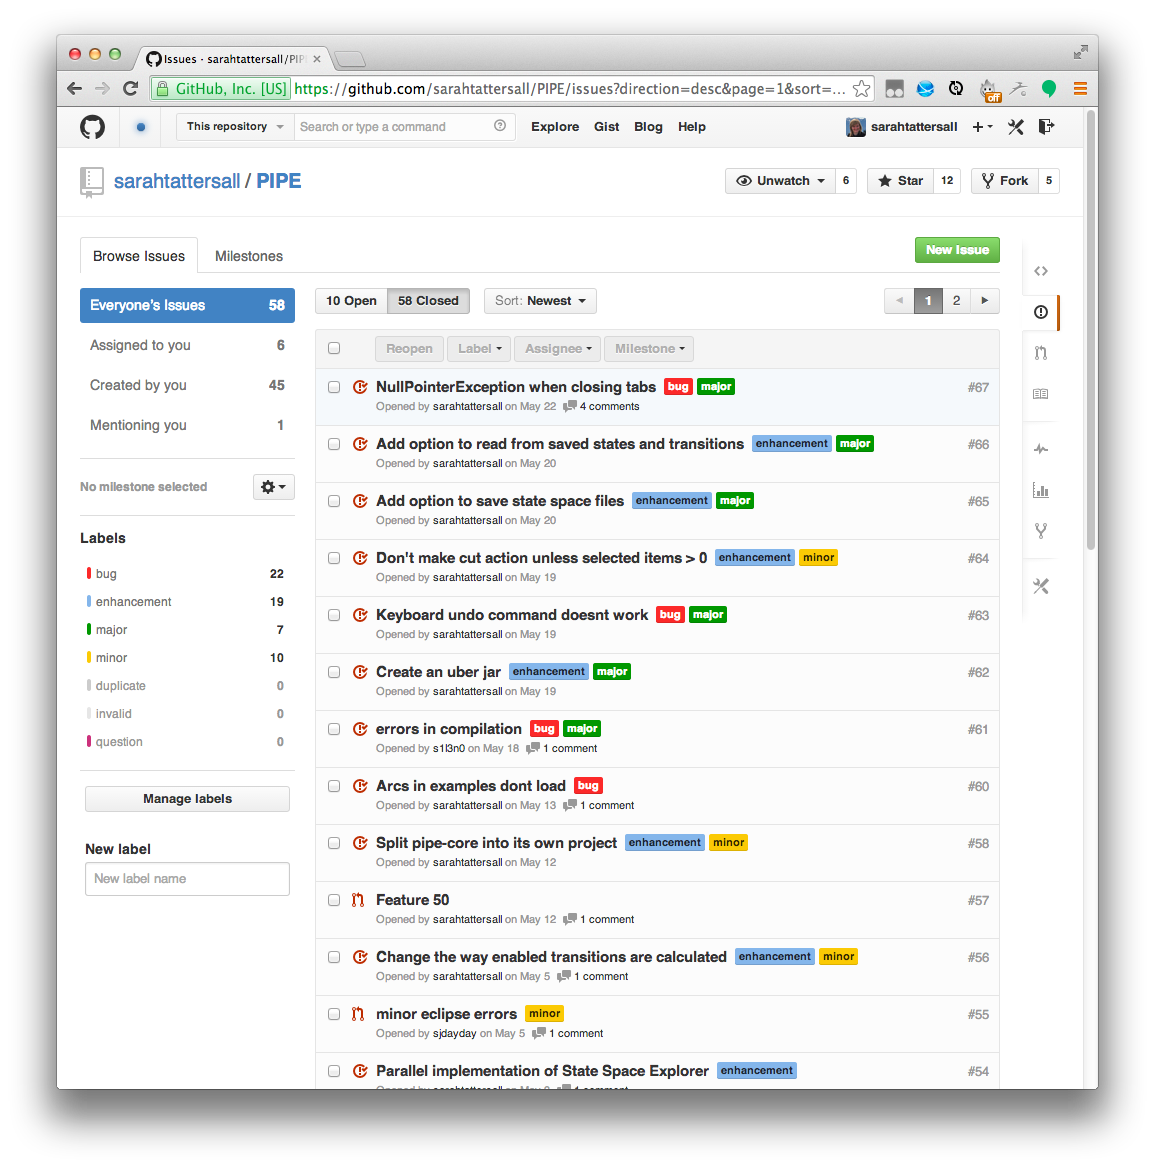
\includegraphics[width=\linewidth]{build/gh_issues.png} 
    \caption{GitHub issue page for PIPE 5 showing a selection of issues that have been raised during the development of PIPE 5. The tags used in PIPE 5 can be seen next to the issues and helped us to prioritise our workload.}
    \label{fig:gh_issues}
\end{center}
\end{figure}

% \begin{figure}[tb]
% \begin{center}
%     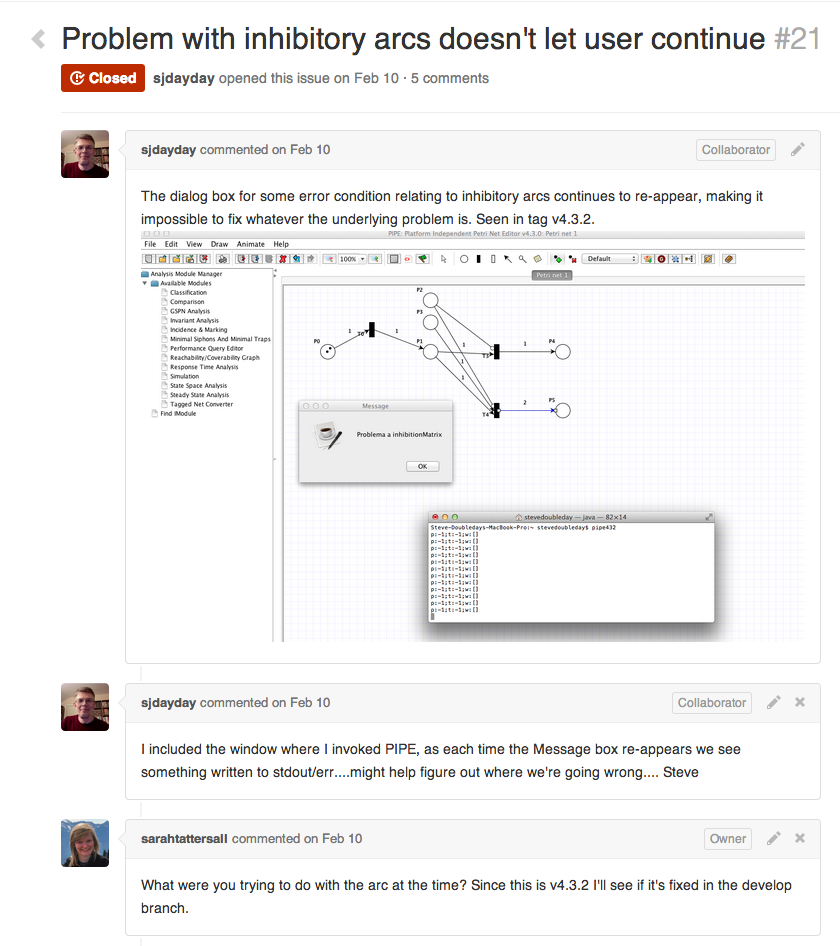
\includegraphics[width=\linewidth]{build/gh_issues_discussion.png} 
%     \caption{A discussion on a GitHub issue of an inhibitor arc bug present in PIPE 4. GitHub allows users to upload screenshots and paste code snippets. Issues and comments are written and displayed in Markdown format for ease of reading.}
%     \label{fig:issue_discussion}
% \end{center}
% \end{figure}
% \normallinespacing

%     \mediumlinespacing
% \begin{figure}[tbp]
% \begin{center}
% \subcaptionbox{Pull request informational page for moving the Travis CI build status to the top of the README.}{
%     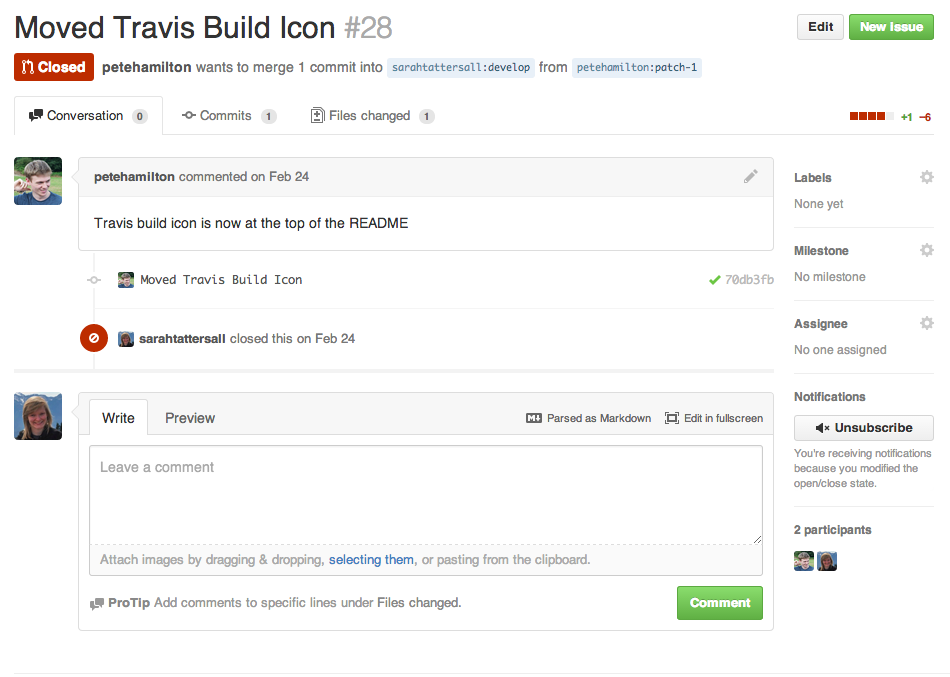
\includegraphics[width=\textwidth]{build/pr.png} 
% }
% \end{center}
% \end{figure}
% \begin{figure}[tbp]
% \begin{center}
% \ContinuedFloat
% \subcaptionbox{Clicking on the commit hash `70db3fb' on the pull request page depicted in (a) leads to this page. Any developer can browse the changes made and optionally comment on any of the lines.}{
%     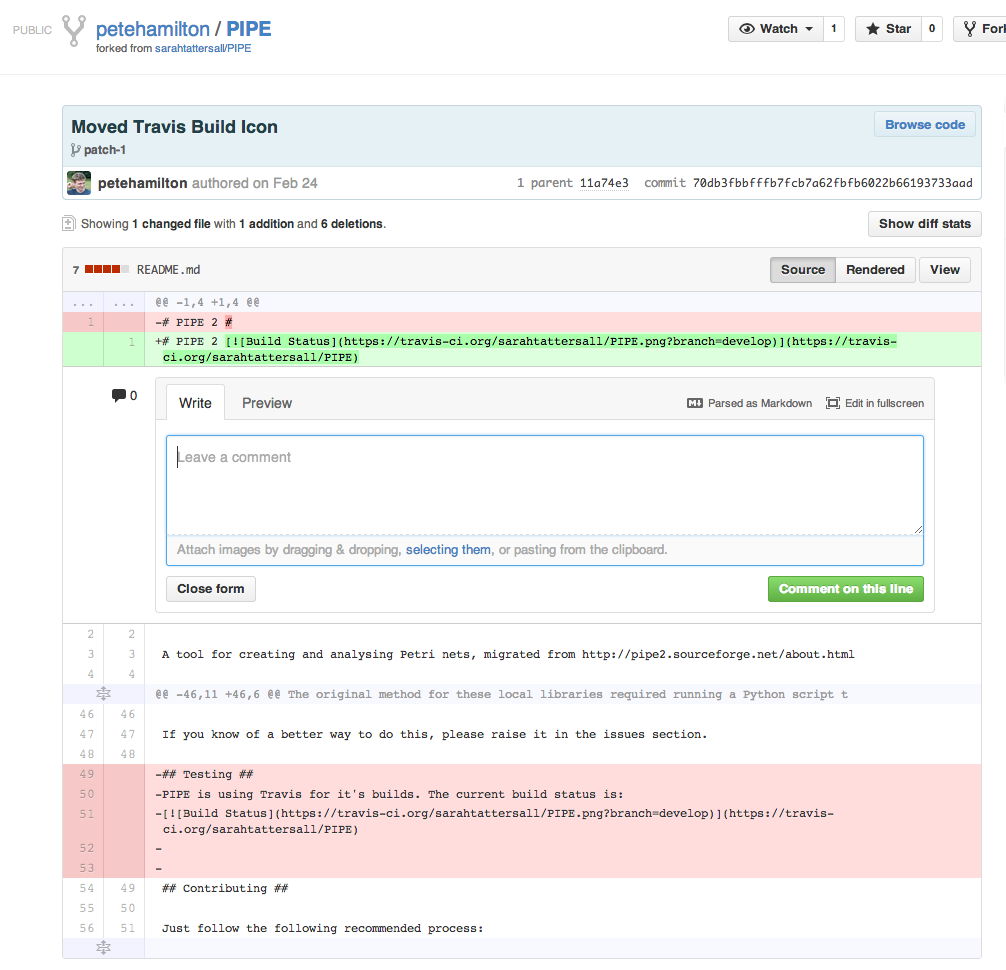
\includegraphics[width=\textwidth]{build/pr_code.png} 
% }
% \caption{A pull request submitted for PIPE where Peter Hamilton forked the project and moved the build status icon to the top of the README.}
% \label{fig:pull_request}
% \end{center}
% \end{figure}
% \normallinespacing

%     \mediumlinespacing
% \begin{figure}[tb]
% \begin{center}
%     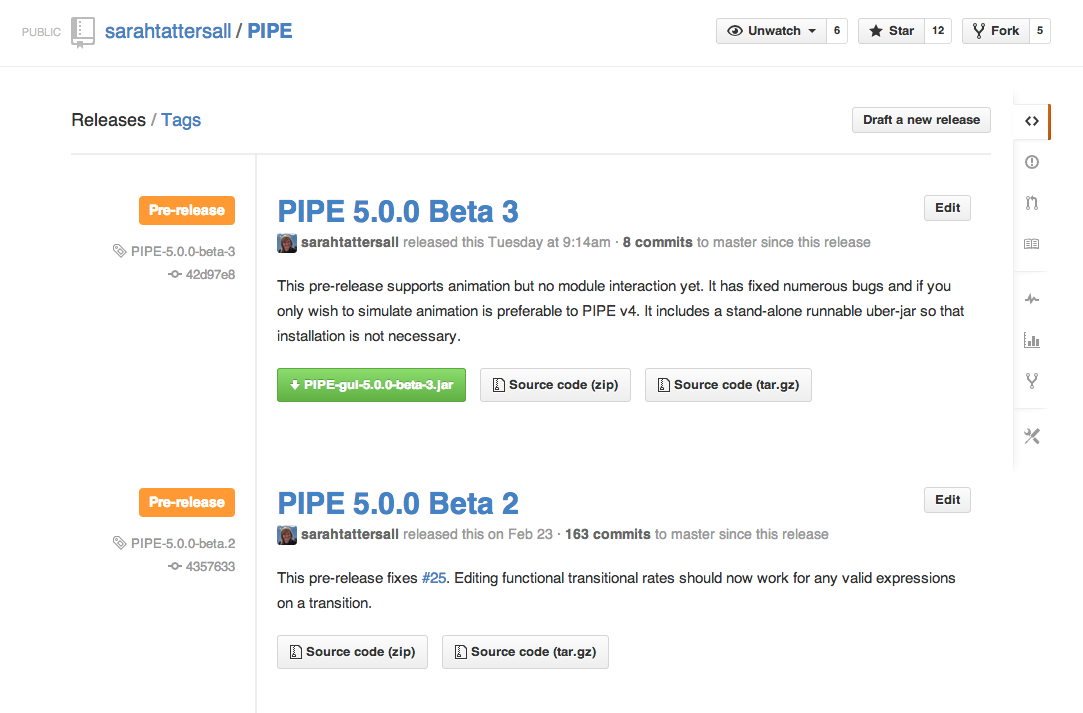
\includegraphics[width=\linewidth]{build/gh_release.png} 
%     \caption{A snippet of the release page on PIPE 5's GitHub repository. Pipe 5.0.0 Beta 3 includes a runnable jar which requires no installation, the user just needs to double click the jar and it opens PIPE 5. This makes the project more accessible to users who do not wish to install the project on their machine.}
%     \label{fig:gh_release}
% \end{center}
% \end{figure}
% \normallinespacing

\begin{figure}[tb]
\begin{center}
    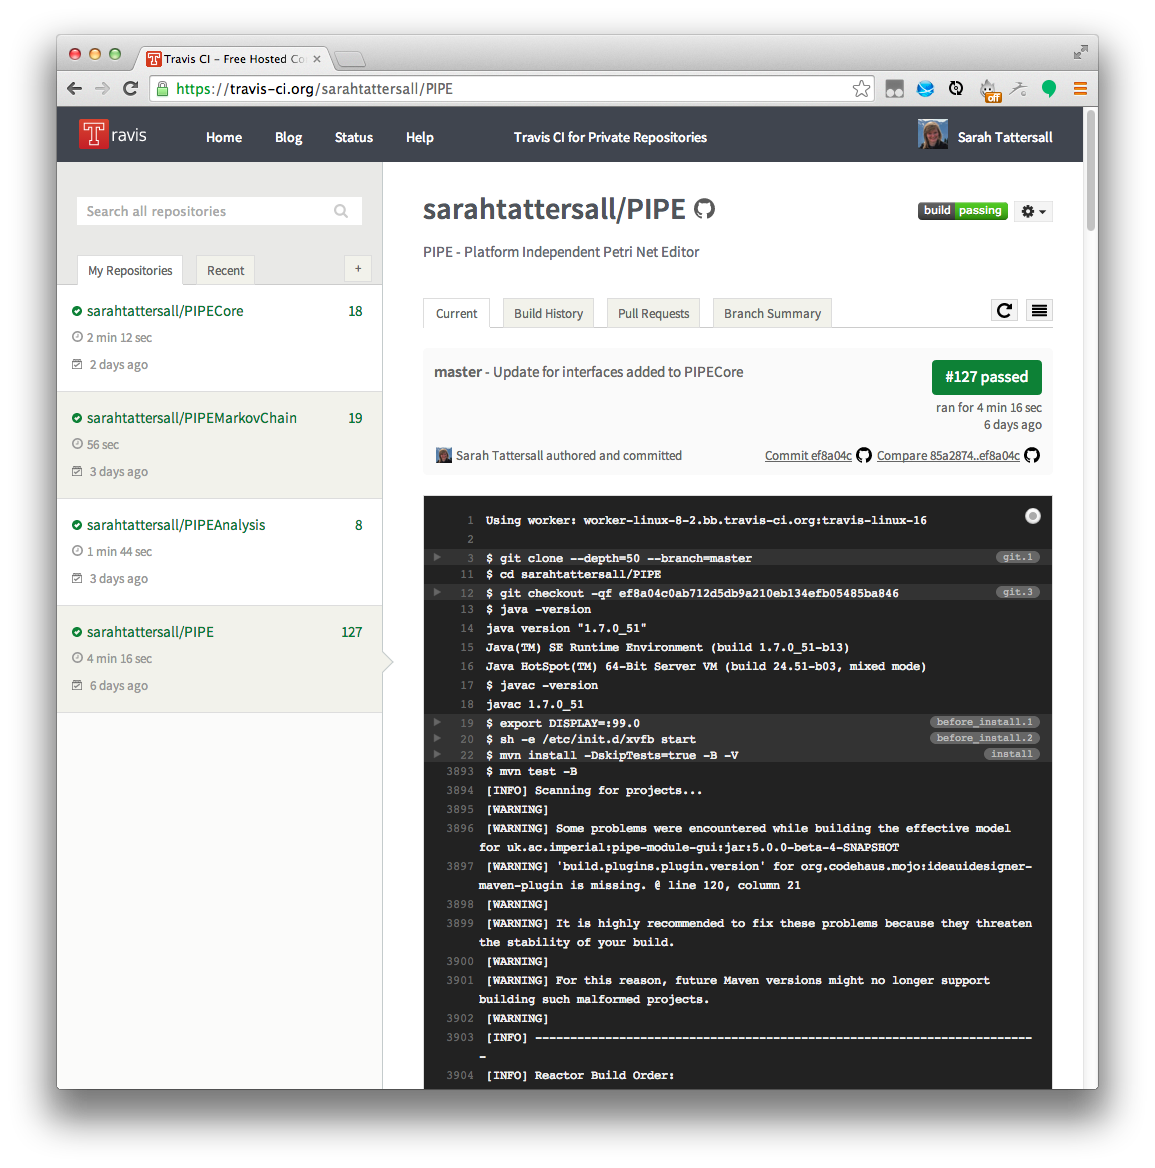
\includegraphics[width=\linewidth]{build/travis_ci.png} 
    \caption{Originally there was no continuous integration server for PIPE 4 which meant that committed changes that broke the build could go undetected. This figure shows the continuous integration server, Travis CI, set up for PIPE 5. The entire console output is shown in the build which is particularly helpful for spotting the cause of an error in failing builds. Builds on Travis CI are triggered by post-commit hooks when pushing changes to GitHub.}
    \label{fig:travis_ci}
\end{center}
\end{figure}

Beyond this we set up a Maven build-system for PIPE 5 to provide a stable cross-platform build process and dependency management system. This overcame problems caused by a collection of user-written build scripts and removed the need to ship external libraries with the codebase.

We made use of Maven build plug-ins to simplify the full release process of PIPE 5 which now involves the following steps:
\begin{itemize} 
    \item Resolving any SNAPSHOT dependencies
     % --- these are dependencies that reference unreleased versions of projects. In PIPE 5 the codebase has been split across multiple repositories so these are the dependencies that reference the other PIPE libraries.
    \item Bumping the version number
     % --- this involves bumping any of the major, minor or patch numbers in the pom for the next release.
    \item Creating a runnable uber-jar
     % --- this creates a jar of PIPE that can simply be run by double clicking on it without having to build the project.
    \item Deploying a project to a Maven repository as an artifact
     % --- all of the repositories involved in PIPE 5 are stored as artifacts on GitHub. This stage allows other developers to reference the projects in their dependencies without manually downloading the jars.
    \item Generate a GitHub release 
    % --- this includes releasing the uber-jar and sources on GitHub for users to download. It appears on the GitHub project release page.
\end{itemize}
The command to execute all of the aforementioned steps can be performed in a single line, which significantly eases the build and release process of PIPE 5:
\begin{lstlisting}
   mvn release:clean release:prepare release:perform.
\end{lstlisting}